\chapter{Just trying...}

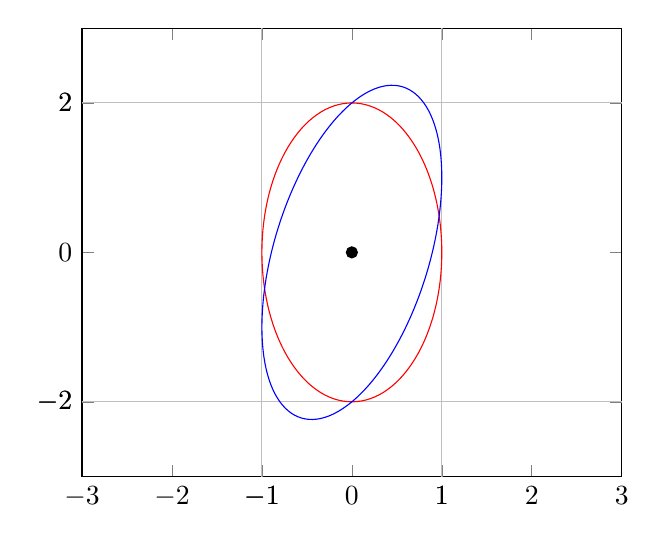
\begin{tikzpicture}
    \begin{axis}[
        xmin=-3,   xmax=3,
        ymin=-3,   ymax=3,
        extra x ticks={-1,1},
        extra y ticks={-2,2},
        extra tick style={grid=major},
    ]
        \draw[red] \pgfextra{
          \pgfpathellipse{\pgfplotspointaxisxy{0}{0}}
            {\pgfplotspointaxisdirectionxy{1}{0}}
            {\pgfplotspointaxisdirectionxy{0}{2}}
          % see also the documentation of 
          % 'axis direction cs' which
          % allows a simpler way to draw this ellipse
        };
        \draw[blue] \pgfextra{
          \pgfpathellipse{\pgfplotspointaxisxy{0}{0}}
            {\pgfplotspointaxisdirectionxy{1}{1}}
            {\pgfplotspointaxisdirectionxy{0}{2}}
        };
        \addplot [only marks,mark=*] coordinates { (0,0) };
    \end{axis}
    \end{tikzpicture}